% !TEX root = ../Thesis.tex
\chapter{Background}

First it is important to explain the various concepts we will be using throughout the thesis. We will cover classical planning, relaxation heuristics and the additive heuristic.

\section{Classical Planning}
\label{sec:my-label}

Planning refers to the process of finding a plan from a given initial state to a goal state. Classical planning refers to the process of finding a plan for a subset of problems, mainly those problems that are static, deterministic and fully observable. These problems are usually described with the use of a planning formalism. Planning formalisms allow us to encode problems in a concise and easily understandable way. Common planning formalisms are STRIPS, ADL, SAS+ and PDDL. For the purpose of this thesis we will focus on STRIPS-style planning tasks enhanced with action costs.  \\

A problem, encoded in STRIPS, is given as input to a planner. The job of the planner is to find a solution (=plan) for the problem. To describe how a planner finds a solution it is useful to introduce a more formal definition of a STRIPS planning task.  \\\\
A STRIPS planning task is a 4-tuple $\Pi = \langle V, I, G, A \rangle$ where:

\begin{itemize}
\setlength\itemsep{0em}
 \item $V$: finite set of state variables 
 \item $I$ $\subseteq V$: the initial state
 \item $G$ $\subseteq V$: the set of goals
 \item $A$: finite set of actions
\end{itemize}

For each action $a \in A$ we also define: 

\begin{itemize}
\setlength\itemsep{0em}
\item $pre(a) \subseteq V$: the preconditions of $a$ 
\item $add(a) \subseteq V$: the add effects of $a$ 
\item $del(a) \subseteq V$: the delete effects of $a$ 
\item $cost(a) \in \mathbb{N}_0$: the cost of $a$ 
\end{itemize}
\newpage

The solution for a STRIPS planning task is a plan from the initial state $I$ to one of the goal states $G$ and an optimal solution is a plan with the lowest cost. To find a solution, the planner induces a state space $\Omega(\Pi) := \langle S,A,cost,T,s_0,S_* \rangle$ where:

\begin{itemize}
\setlength\itemsep{0em}
\item $S$: set of states = $2^V$ = (power set of $V$)
\item $A$: actions as defined in $\Pi$ 
\item $cost$: costs as defined in $\Pi$ 
\item $T$: transitions $s \xrightarrow[\text{}]{\text{a}} s'$ for states $s$, $s’$ and action $a$ iff: 
\begin{itemize}
\setlength\itemsep{0em}
\item $pre(a) \in s$ (preconditions satisfied)
\item $s' = (s \setminus del(a)) \cup add(a)$ (delete and add effects are applied)
\end{itemize}
\item $s_0$: initial state $s_0 = I$
\item $S_*$: set of goal states $s \in S_*$ for state $s$ iff $G \subseteq s$ (goals reached) \quad\quad\quad\quad\quad\quad\quad
\end{itemize}
 
A planner can then find a solution for the state space $\Omega$ using different search algorithms. As they are generally faster heuristic based search algorithms such as A* are usually used. The question now is how heuristic values can be derived from STRIPS encodings. 



\section{Relaxation Heuristics}

There are many different ways of deriving heuristic values from STRIPS encodings, one of the most successful approaches is to consider a relaxed version of the planning task. \\\\
A relaxed version of a planning task is identical to the original except for one important difference, for every action $a \subseteq A$ the delete effects $del(a)$ are ignored. This means that, in a relaxed planning task, applying an action to a state always leads to a state where more or an equal number of state variables are true. This trivializes the search significantly as applying any possible action at any possible step of the search is certain to at the very least not undo any progress we have made. To put it differently, every action brings us closer to the goal or it keeps us at a consistent distance to the goal, we never take a step backwards. \\\\
To define a relaxed planning task more formally let us first introduce a relaxed version $a^+$ of an action $a$ with: 

\begin{itemize}
\setlength\itemsep{0em}
\item $pre(a^+) = pre(a)$
\item $add(a^+) = add(a)$
\item $cost(a^+) = cost(a)$ 
\item $del(a^+) = \emptyset$
\end{itemize}

 

A relaxed version $\Pi^+$ of a STRIPS planning task $\Pi = \langle V, I, G, A \rangle$ is defined as: 

\begin{equation*}
    \Pi^+ := \langle V, I, G, \{a^+|a \in A\} \rangle
\end{equation*}
\newpage
Let $s^0,...,s^n \in S$ be states and $a^1,...,a^n \in A$ be actions such that $s^0\xrightarrow[\text{}]{a^1} s^1,...,s^n^-^1\xrightarrow[\text{}]{a^n} s^n$. A plan is a sequence of actions $\pi = \langle a_1 ,$...$, a_n \rangle$ that leads from $s^0$ to $s^n$. The cost of a plan is defined as $cost(\pi) = \sum_{i = 1}^{n} cost(a_i)$, the optimal plan $\pi^*$ is the plan with minimum $cost(\pi)$ among all plans $\pi \in \Lambda$, with $\Lambda$ being the set of all plans from a given $s^0$ and $s^n$. A plan for $\Pi^+$ is denoted by $\pi^+$ which is also called a relaxed plan for $\Pi$. $h^+(\Pi)$ denotes the cost of an optimal plan for $\Pi^+$ and $h^+(s)$ denotes the cost of an optimal plan for $\Pi^+$ starting in state $s \subseteq S$. $h^+$ is called the optimal relaxation heuristic.\\

 

The question now is how this relaxed version $\Pi^+$ of a STRIPS planning task $\Pi$ helps us find informed heuristic values for $\Pi$. The general idea is to use the cost of an optimal relaxed plan $h^+(s)$ as heuristic values for each state $s \subseteq S$. Unfortunately, there is a catch with this idea. The computation of $h^+$ is NP-hard. It is not feasible to use $h^+$ as heuristic values since the computation would take too much time, therefore we have to approximate $h^+$ in a time efficient manner. The domain of relaxation heuristics cover different ways of approximating $h^+$. One such form of approximation is the additive heuristic. 


\section{Additive Heuristic}

The additive heuristic ($h^a^d^d$) is a relaxation heuristic and therefore it has the central goal of approximating $h^+$ in a time efficient manner. In order to properly explain how $h^a^d^d$ works, we first introduce the concept of a relaxed planning graph. 

\subsection{Relaxed Planning Graph}

A relaxed planning graph is a graphical representation of the variables in $\Pi^+$ which can be reached and how they can be reached. To explain how a relaxed planning graph works and what information is displayed let us first look at the following example. Consider the relaxed planning task $\Pi^+ = \langle V, I, G, A \rangle$ with:

\begin{itemize}
\setlength\itemsep{0em}
\item $V = \{a,b,c,d,e,f,g,h\}$
\item $I = \{a\}$
\item $G = \{c,d,e,f,g\}$ 
\item $A = \{a_1,a_2,a_3,a_4,a_5,a_6\}$
\item $a_1 = a \xrightarrow[\text{}]{\text{3}} b,c$
\item $a_2 = a,c \xrightarrow[\text{}]{\text{1}} d$
\item $a_3 = b,c \xrightarrow[\text{}]{\text{1}} e$
\item $a_4 = b \xrightarrow[\text{}]{\text{1}} f$
\item $a_5 = d \xrightarrow[\text{}]{\text{1}} e,f$
\item $a_6 = d \xrightarrow[\text{}]{\text{1}} g$
\end{itemize}
\newpage
The relaxed planning graph for this task now looks as follows:
\begin{figure}
\centering
% -*- mode: latex; coding: utf-8 -*-

\subtitle{}
\date{April 29, 2020}

%% TODO: This needs to be shortened a bit. In 2013, this lecture was
%% 5-10 minutes too long (I managed it in one session but ran over)
%% without being too slow or too fast. We can probably get rid of the
%% 15-puzzle stuff, moving it to the exercises to make some time. And
%% a not-RPG-centric description of h^max/h^add/h^FF could probably
%% also be done faster than the current RPG-centric one.

\usetikzlibrary{shapes}

\tikzstyle{relaxed planning graph}=[draw,inner sep=0pt,font=\small]
\tikzstyle{rpg square}=[relaxed planning graph,minimum size=0.52cm,rectangle]
\tikzstyle{rpg circle}=[relaxed planning graph,minimum size=0.52cm,circle]

\tikzstyle{prop}=        [rpg circle,fill=yellow]
\tikzstyle{notthere}=    [color=gray!15,fill=gray!5]
\tikzstyle{operator}=    [rpg square,fill=blue!40]
\tikzstyle{selected}=[fill=cyan]

\tikzstyle{goalachieved}=[fill=red!50]
\tikzstyle{solved} = [fill=green!30]
\tikzstyle{assignedprop}=[rpg circle,fill=orange!40]
\tikzstyle{assignedoperator}=[rpg square,fill=orange!40]

\tikzstyle{idle}=[thin]
\tikzstyle{nonidle}=[thin]
\tikzstyle{arc selected}=[color=cyan,very thick]

\newcommand{\markplusone}[1]{\path (#1) +(-0.04cm,0.28cm) node {\tiny $+1$};}
\newcommand{\markopnode}[3][0.35cm]{\path (#2) +(0cm,#1) node {\tiny
    \ensuremath{#3}};}
\newcommand{\markopnodeff}[3][0.30cm]{\path (#2) +(0cm,#1) node {\tiny
    \ensuremath{#3}};}
\newcommand{\markopcost}[2]{\path (#1) +(0.45cm,0.15cm) node {\tiny $+#2$};}

\newcommand{\pre}{\ensuremath{\textit{pre}}}
\newcommand{\add}{\ensuremath{\textit{add}}}
\newcommand{\del}{\ensuremath{\textit{del}}}
\newcommand{\relaxation}[1]{\ensuremath{#1^+}}
\newcommand{\hplus}{\ensuremath{h^+}}
\newcommand{\hmax}{\ensuremath{h^{\textup{max}}}}
\newcommand{\hadd}{\ensuremath{h^{\textup{add}}}}
\newcommand{\hff}{\ensuremath{h^{\textup{FF}}}}


\begin{frame}{}
  %% TODO: Got rid of centering to avoid the graph jumping.
  %% Should find a better solution for this.
  %% \begin{center}
    \begin{tikzpicture}
      \pgfsetxvec{\pgfpoint{2.77cm}{0.0cm}}
      \pgfsetyvec{\pgfpoint{0.0cm}{0.87cm}}
      %% variable layer 0
      \only<1->{
        \node[prop] at (0.0,7.0) (a0) {$a^0$};
        \node[prop,notthere] at (0.0,6.0) (b0) {$b^0$};
        \node[prop,notthere] at (0.0,5.0) (c0) {$c^0$};
        \node[prop,notthere] at (0.0,4.0) (d0) {$d^0$};
        \node[prop,notthere] at (0.0,3.0) (e0) {$e^0$};
        \node[prop,notthere] at (0.0,2.0) (f0) {$f^0$};
        \node[prop,notthere] at (0.0,1.0) (g0) {$g^0$};
        \node[prop,notthere] at (0.0,0.0) (h0) {$h^0$};
      }
      %% action layer 1
      \only<2->{
        %% action a_1
        \node[operator] at (0.5,6.5) (o1-1) {$a_1$};
        \draw[->,nonidle] (a0)--(o1-1);
      }
      %% variable layer 1
      \only<3->{
        \node[prop] at (1.0,7.0) (a1) {$a^1$};
        \node[prop] at (1.0,6.0) (b1) {$b^1$};
        \node[prop] at (1.0,5.0) (c1) {$c^1$};
        \node[prop,notthere] at (1.0,4.0) (d1) {$d^1$};
        \node[prop,notthere] at (1.0,3.0) (e1) {$e^1$};
        \node[prop,notthere] at (1.0,2.0) (f1) {$f^1$};
        \node[prop,notthere] at (1.0,1.0) (g1) {$g^1$};
        \node[prop,notthere] at (1.0,0.0) (h1) {$h^1$};
        %% idle arcs
        \draw[->,idle] (a0)--(a1);
        \draw[->,idle,notthere] (b0)--(b1);
        \draw[->,idle,notthere] (c0)--(c1);
        \draw[->,idle,notthere] (d0)--(d1);
        \draw[->,idle,notthere] (e0)--(e1);
        \draw[->,idle,notthere] (f0)--(f1);
        \draw[->,idle,notthere] (g0)--(g1);
        \draw[->,idle,notthere] (h0)--(h1);
        %% effect arcs
        \draw[->,nonidle] (o1-1)--(b1);
        \draw[->,nonidle] (o1-1)--(c1);
      }
      %% action layer 2
      \only<4->{
        %% action a_1
        \node[operator] at (1.5,6.5) (o1-2) {$a_1$};
        \draw[->,nonidle] (a1)--(o1-2);
        %% action a_2
        \node[operator] at (1.5,5.5) (o2-2) {$a_2$};
        \draw[->,nonidle] (a1)--(o2-2);
        \draw[->,nonidle] (c1)--(o2-2);
        %% action a_3
        \node[operator] at (1.5,4.5) (o3-2) {$a_3$};
        \draw[->,nonidle] (b1)--(o3-2);
        \draw[->,nonidle] (c1)--(o3-2);
        %% action a_4
        \node[operator] at (1.5,3.5) (o4-2) {$a_4$};
        \draw[->,nonidle] (b1)--(o4-2);
      }
      %% variable layer 2
      \only<5->{
        \node[prop] at (2.0,7.0) (a2) {$a^2$};
        \node[prop] at (2.0,6.0) (b2) {$b^2$};
        \node[prop] at (2.0,5.0) (c2) {$c^2$};
        \node[prop] at (2.0,4.0) (d2) {$d^2$};
        \node[prop] at (2.0,3.0) (e2) {$e^2$};
        \node[prop] at (2.0,2.0) (f2) {$f^2$};
        \node[prop,notthere] at (2.0,1.0) (g2) {$g^2$};
        \node[prop,notthere] at (2.0,0.0) (h2) {$h^2$};
        %% effect arcs
        \draw[->,nonidle] (o1-2)--(b2);
        \draw[->,nonidle] (o1-2)--(c2);
        \draw[->,nonidle] (o2-2)--(d2);
        \draw[->,nonidle] (o3-2)--(e2);
        \draw[->,nonidle] (o4-2)--(f2);
        %% idle arcs
        \draw[->,idle] (a1)--(a2);
        \draw[->,idle] (b1)--(b2);
        \draw[->,idle] (c1)--(c2);
        \draw[->,idle,notthere] (d1)--(d2);
        \draw[->,idle,notthere] (e1)--(e2);
        \draw[->,idle,notthere] (f1)--(f2);
        \draw[->,idle,notthere] (g1)--(g2);
        \draw[->,idle,notthere] (h1)--(h2);
      }
      %% action layer 3
      \only<6->{
        %% action a_1
        \node[operator] at (2.5,6.5) (o1-3) {$a_1$};
        \draw[->,nonidle] (a2)--(o1-3);
        %% action a_2
        \node[operator] at (2.5,5.5) (o2-3) {$a_2$};
        \draw[->,nonidle] (a2)--(o2-3);
        \draw[->,nonidle] (c2)--(o2-3);
        %% action a_3
        \node[operator] at (2.5,4.5) (o3-3) {$a_3$};
        \draw[->,nonidle] (b2)--(o3-3);
        \draw[->,nonidle] (c2)--(o3-3);
        %% action a_4
        \node[operator] at (2.5,3.5) (o4-3) {$a_4$};
        \draw[->,nonidle] (b2)--(o4-3);
        %% action a_5
        \node[operator] at (2.5,2.5) (o5-3) {$a_5$};
        \draw[->,nonidle] (d2)--(o5-3);
        %% action a_6
        \node[operator] at (2.5,1.5) (o6-3) {$a_6$};
        \draw[->,nonidle] (d2)--(o6-3);
      }
      %% variable layer 3
      \only<7->{
        \node[prop] at (3.0,7.0) (a3) {$a^3$};
        \node[prop] at (3.0,6.0) (b3) {$b^3$};
        \node[prop] at (3.0,5.0) (c3) {$c^3$};
        \node[prop] at (3.0,4.0) (d3) {$d^3$};
        \node[prop] at (3.0,3.0) (e3) {$e^3$};
        \node[prop] at (3.0,2.0) (f3) {$f^3$};
        \node[prop] at (3.0,1.0) (g3) {$g^3$};
        \node[prop,notthere] at (3.0,0.0) (h3) {$h^3$};
        %% effect arcs
        \draw[->,nonidle] (o1-3)--(b3);
        \draw[->,nonidle] (o1-3)--(c3);
        \draw[->,nonidle] (o2-3)--(d3);
        \draw[->,nonidle] (o3-3)--(e3);
        \draw[->,nonidle] (o4-3)--(f3);
        \draw[->,nonidle] (o5-3)--(e3);
        \draw[->,nonidle] (o5-3)--(f3);
        \draw[->,nonidle] (o6-3)--(g3);
        %% idle arcs
        \draw[->,idle] (a2)--(a3);
        \draw[->,idle] (b2)--(b3);
        \draw[->,idle] (c2)--(c3);
        \draw[->,idle] (d2)--(d3);
        \draw[->,idle] (e2)--(e3);
        \draw[->,idle] (f2)--(f3);
        \draw[->,idle,notthere] (g2)--(g3);
        \draw[->,idle,notthere] (h2)--(h3);
      }
      \only<beamer:8|handout:0>{
        \node[prop,goalachieved] at (3.0,5.0) (c3) {$c^3$};
        \node[prop,goalachieved] at (3.0,4.0) (d3) {$d^3$};
        \node[prop,goalachieved] at (3.0,3.0) (e3) {$e^3$};
        \node[prop,goalachieved] at (3.0,2.0) (f3) {$f^3$};
        \node[prop,goalachieved] at (3.0,1.0) (g3) {$g^3$};
      }
      \only<9->{
        \node[operator,goalachieved] at (3.5,3.0) (G) {$G$};
        \draw[->,nonidle] (c3)--(G);
        \draw[->,nonidle] (d3)--(G);
        \draw[->,nonidle] (e3)--(G);
        \draw[->,nonidle] (f3)--(G);
        \draw[->,nonidle] (g3)--(G);
      }
    \end{tikzpicture}
  %% \end{center}
\end{frame}

\caption{Relaxed planning graph}
\label{fig:machine}
\end{figure}
\\The graph is structured in a series of variable layers $V^i$ and action layers $A^i$ where:

\begin{itemize}
\setlength\itemsep{0em}
\item variable layer $V^0$ contains the variable vertex $v^0$ for all $v \in I$
\item action layer $A^i^+^1$ contains the action vertex $a^i^+^1$ for action $a$ if $V^i$ contains the vertex $v^i$ for all $v \in pre(a)$
\item variable layer $V^i^+^1$ contains the variable vertex $v^i^+^1$ if the previous variable layer contains $v^i$ or the previous action layer contains $a^i^+^1$ with $v \in add(a)$
\item goal vertices $G^i$ are reached if $v^i \in V^i$ for all $v \in G$
\item directed edges:
\begin{itemize}
\setlength\itemsep{0em}
\item from $v^i$ to $a^i^+^1$ if $v \in pre(a)$ (precondition edges)
\item from $a^i$ to $v^i$ if $v \in add(a)$ (effect edges)
\item from $v^i$ to $G^i$ if $v \in G$ (goal edges)
\item from $v^i$ to $v^i^+^1$ (no-op edges) \quad\quad\quad\quad\quad\quad\quad\quad\quad\quad\quad\quad\quad\quad\quad\quad\quad\quad\quad\quad
\end{itemize}
\end{itemize}

We can now use this relaxed planning graph to help us understand how the additive heuristic works.

\subsection{Understanding the Additive Heuristic}

The central goal of all relaxation heuristics is to approximate $h^+$. We can think of $h^+$ as the optimal sequence of actions to reach the goal vertex $G$ form variable layer $V^0$. In order to approximate $h^+$, $h^a^d^d$ annotates all vertices and all actions with numerical values. These values estimate the cost to reach a vertex or to reach all preconditions of an action. We use $g_s(v)$ to denote the estimate cost of achieving variable $v \in V$ from state $s \subseteq S$, and $g_s(a)$ to denote the estimate cost of achieving all preconditions of action $a \in A$ from state $s \subseteq S$. $h^a^d^d$ updates the variable and action values according to the following equations:

\begin{equation}
 g_s(v) = 
  \begin{cases} 
   0 & \text{if } v \in s \\
   \text{min}_a_\in_A_|_v_\in_a_d_d_(_a_) [cost(a) + g_s(a)]       & \text{otherwise } 
  \end{cases}
\end{equation}

\begin{equation}
    g_s(a) = \sum_{v \in pre(a)}^{} g_s(v)
\end{equation}

Note that if $v \in pre(a) := \emptyset$ then $\sum_{v \in pre(a)}^{} g_s(v) := 0$ and if $a \in A | v \in add(a) := \emptyset$ then $\text{min}_a_\in_A_|_v_\in_a_d_d_(_a_) [g_s(a)] := \infty$.\\

$h^a^d^d$ makes the fundamental assumption that in order to reach action $a \in A$, all preconditions $pre(a)$ of $a$ must be reached independently of another, hence the summation in (2.2). This makes $h^a^d^d$ a pessimistic algorithm, as it assumes the worst case scenario of needing to reach all precondition variables independently of another. Now lets look at a version of the previous relaxed planning graph, but this time with the annotated $h^a^d^d$ cost values:

\begin{figure}
\centering
% -*- mode: latex; coding: utf-8 -*-

\subtitle{}
\date{April 29, 2020}

%% TODO: This needs to be shortened a bit. In 2013, this lecture was
%% 5-10 minutes too long (I managed it in one session but ran over)
%% without being too slow or too fast. We can probably get rid of the
%% 15-puzzle stuff, moving it to the exercises to make some time. And
%% a not-RPG-centric description of h^max/h^add/h^FF could probably
%% also be done faster than the current RPG-centric one.
% !TEX root = ../Thesis.tex

\usetikzlibrary{shapes}

\tikzstyle{relaxed planning graph}=[draw,inner sep=0pt,font=\small]
\tikzstyle{rpg square}=[relaxed planning graph,minimum size=0.52cm,rectangle]
\tikzstyle{rpg circle}=[relaxed planning graph,minimum size=0.52cm,circle]


\tikzstyle{prop}=        [rpg circle,fill=yellow]
\tikzstyle{notthere}=    [color=gray!15,fill=gray!5]
\tikzstyle{operator}=    [rpg square,fill=blue!40]
\tikzstyle{solved} = [fill=green!30]
\tikzstyle{selected}=[fill=cyan]

\tikzstyle{goalachieved}=[fill=red!50]
\tikzstyle{assignedprop}=[rpg circle,fill=orange!40]
\tikzstyle{assignedoperator}=[rpg square,fill=orange!40]

\tikzstyle{idle}=[thin]
\tikzstyle{nonidle}=[thin]
\tikzstyle{arc selected}=[color=cyan,very thick]

\newcommand{\markplusone}[1]{\path (#1) +(-0.04cm,0.28cm) node {\tiny $+1$};}
\newcommand{\markopnode}[3][0.35cm]{\path (#2) +(0cm,#1) node {\tiny
    \ensuremath{#3}};}
\newcommand{\markopnodeff}[3][0.30cm]{\path (#2) +(0cm,#1) node {\tiny
    \ensuremath{#3}};}
\newcommand{\markopcost}[2]{\path (#1) +(0.45cm,0.15cm) node {\tiny $+#2$};}

\newcommand{\pre}{\ensuremath{\textit{pre}}}
\newcommand{\add}{\ensuremath{\textit{add}}}
\newcommand{\del}{\ensuremath{\textit{del}}}
\newcommand{\relaxation}[1]{\ensuremath{#1^+}}
\newcommand{\hplus}{\ensuremath{h^+}}
\newcommand{\hmax}{\ensuremath{h^{\textup{max}}}}
\newcommand{\hadd}{\ensuremath{h^{\textup{add}}}}
\newcommand{\hff}{\ensuremath{h^{\textup{FF}}}}

\begin{minipage}[t]{.7\linewidth}
\vspace{0pt}
\begin{center}
\centering
\begin{frame}{}
  %% TODO: Got rid of centering to avoid the graph jumping.
  %% Should find a better solution for this.
  %% \begin{center}
    \begin{tikzpicture}
      \pgfsetxvec{\pgfpoint{2.77cm}{0.0cm}}
      \pgfsetyvec{\pgfpoint{0.0cm}{0.87cm}}
      %% variable layer 0
      \only<1->{
        \node[prop, solved] at (0.0,7.0) (a0) {0};
        \node[prop,notthere] at (0.0,6.0) (b0) {$b^0$};
        \node[prop,notthere] at (0.0,5.0) (c0) {$c^0$};
        \node[prop,notthere] at (0.0,4.0) (d0) {$d^0$};
        \node[prop,notthere] at (0.0,3.0) (e0) {$e^0$};
        \node[prop,notthere] at (0.0,2.0) (f0) {$f^0$};
        \node[prop,notthere] at (0.0,1.0) (g0) {$g^0$};
        \node[prop,notthere] at (0.0,0.0) (h0) {$h^0$};
      }
      %% action layer 1
      \only<2->{
        %% action a_1
        \node[operator, solved] at (0.5,6.5) (o1-1) {0};
        \draw[->,nonidle] (a0)--(o1-1);
      }
      %% variable layer 1
      \only<3->{
        \node[prop, solved] at (1.0,7.0) (a1) {0};
        \node[prop, solved] at (1.0,6.0) (b1) {3};
        \node[prop, solved] at (1.0,5.0) (c1) {3};
        \node[prop,notthere] at (1.0,4.0) (d1) {$d^1$};
        \node[prop,notthere] at (1.0,3.0) (e1) {$e^1$};
        \node[prop,notthere] at (1.0,2.0) (f1) {$f^1$};
        \node[prop,notthere] at (1.0,1.0) (g1) {$g^1$};
        \node[prop,notthere] at (1.0,0.0) (h1) {$h^1$};
        %% idle arcs
        \draw[->,idle] (a0)--(a1);
        \draw[->,idle,notthere] (b0)--(b1);
        \draw[->,idle,notthere] (c0)--(c1);
        \draw[->,idle,notthere] (d0)--(d1);
        \draw[->,idle,notthere] (e0)--(e1);
        \draw[->,idle,notthere] (f0)--(f1);
        \draw[->,idle,notthere] (g0)--(g1);
        \draw[->,idle,notthere] (h0)--(h1);
        %% effect arcs
        \draw[->,nonidle] (o1-1)--(b1);
        \draw[->,nonidle] (o1-1)--(c1);
      }
      %% action layer 2
      \only<4->{
        %% action a_1
        \node[operator, solved] at (1.5,6.5) (o1-2) {0};
        \draw[->,nonidle] (a1)--(o1-2);
        %% action a_2
        \node[operator, solved] at (1.5,5.5) (o2-2) {3};
        \draw[->,nonidle] (a1)--(o2-2);
        \draw[->,nonidle] (c1)--(o2-2);
        %% action a_3
        \node[operator, solved] at (1.5,4.5) (o3-2) {6};
        \draw[->,nonidle] (b1)--(o3-2);
        \draw[->,nonidle] (c1)--(o3-2);
        %% action a_4
        \node[operator, solved] at (1.5,3.5) (o4-2) {3};
        \draw[->,nonidle] (b1)--(o4-2);
      }
      %% variable layer 2
      \only<5->{
        \node[prop, solved] at (2.0,7.0) (a2) {0};
        \node[prop, solved] at (2.0,6.0) (b2) {3};
        \node[prop, solved] at (2.0,5.0) (c2) {3};
        \node[prop, solved] at (2.0,4.0) (d2) {4};
        \node[prop, solved] at (2.0,3.0) (e2) {7};
        \node[prop, solved] at (2.0,2.0) (f2) {4};
        \node[prop,notthere] at (2.0,1.0) (g2) {$g^2$};
        \node[prop,notthere] at (2.0,0.0) (h2) {$h^2$};
        %% effect arcs
        \draw[->,nonidle] (o1-2)--(b2);
        \draw[->,nonidle] (o1-2)--(c2);
        \draw[->,nonidle] (o2-2)--(d2);
        \draw[->,nonidle] (o3-2)--(e2);
        \draw[->,nonidle] (o4-2)--(f2);
        %% idle arcs
        \draw[->,idle] (a1)--(a2);
        \draw[->,idle] (b1)--(b2);
        \draw[->,idle] (c1)--(c2);
        \draw[->,idle,notthere] (d1)--(d2);
        \draw[->,idle,notthere] (e1)--(e2);
        \draw[->,idle,notthere] (f1)--(f2);
        \draw[->,idle,notthere] (g1)--(g2);
        \draw[->,idle,notthere] (h1)--(h2);
      }
      %% action layer 3
      \only<6->{
        %% action a_1
        \node[operator, solved] at (2.5,6.5) (o1-3) {0};
        \draw[->,nonidle] (a2)--(o1-3);
        %% action a_2
        \node[operator, solved] at (2.5,5.5) (o2-3) {3};
        \draw[->,nonidle] (a2)--(o2-3);
        \draw[->,nonidle] (c2)--(o2-3);
        %% action a_3
        \node[operator, solved] at (2.5,4.5) (o3-3) {6};
        \draw[->,nonidle] (b2)--(o3-3);
        \draw[->,nonidle] (c2)--(o3-3);
        %% action a_4
        \node[operator, solved] at (2.5,3.5) (o4-3) {3};
        \draw[->,nonidle] (b2)--(o4-3);
        %% action a_5
        \node[operator, solved] at (2.5,2.5) (o5-3) {4};
        \draw[->,nonidle] (d2)--(o5-3);
        %% action a_6
        \node[operator, solved] at (2.5,1.5) (o6-3) {4};
        \draw[->,nonidle] (d2)--(o6-3);
      }
      %% variable layer 3
      \only<7->{
        \node[prop, solved] at (3.0,7.0) (a3) {0};
        \node[prop, solved] at (3.0,6.0) (b3) {3};
        \node[prop, solved] at (3.0,5.0) (c3) {3};
        \node[prop, solved] at (3.0,4.0) (d3) {4};
        \node[prop, solved] at (3.0,3.0) (e3) {7};
        \node[prop, solved] at (3.0,2.0) (f3) {4};
        \node[prop, solved] at (3.0,1.0) (g3) {5};
        \node[prop,notthere] at (3.0,0.0) (h3) {$h^3$};
        %% effect arcs
        \draw[->,nonidle] (o1-3)--(b3);
        \draw[->,nonidle] (o1-3)--(c3);
        \draw[->,nonidle] (o2-3)--(d3);
        \draw[->,nonidle] (o3-3)--(e3);
        \draw[->,nonidle] (o4-3)--(f3);
        \draw[->,nonidle] (o5-3)--(e3);
        \draw[->,nonidle] (o5-3)--(f3);
        \draw[->,nonidle] (o6-3)--(g3);
        %% idle arcs
        \draw[->,idle] (a2)--(a3);
        \draw[->,idle] (b2)--(b3);
        \draw[->,idle] (c2)--(c3);
        \draw[->,idle] (d2)--(d3);
        \draw[->,idle] (e2)--(e3);
        \draw[->,idle] (f2)--(f3);
        \draw[->,idle,notthere] (g2)--(g3);
        \draw[->,idle,notthere] (h2)--(h3);
      }
      \only<beamer:8|handout:0>{
        \node[prop,solved] at (3.0,5.0) (c3) {3};
        \node[prop,solved] at (3.0,4.0) (d3) {4};
        \node[prop,solved] at (3.0,3.0) (e3) {5};
        \node[prop,solved] at (3.0,2.0) (f3) {4};
        \node[prop,solved] at (3.0,1.0) (g3) {5};
      }
      \only<9->{
        \node[operator,goalachieved] at (3.5,3.0) (G) {21};
        \draw[->,nonidle] (c3)--(G);
        \draw[->,nonidle] (d3)--(G);
        \draw[->,nonidle] (e3)--(G);
        \draw[->,nonidle] (f3)--(G);
        \draw[->,nonidle] (g3)--(G);
      }
    \end{tikzpicture}
    $\hadd(\{a\}) = 21$
  %% \end{center}
\end{frame}
\end{center}
\end{minipage}
\caption{Relaxed planning graph with $h^a^d^d$ values}
\label{fig:machine}
\end{figure}
We will not cover how the relaxed planning graph updates its cost values layer by layer, the relaxed planning graph serves us as an intuitive visual aid, the underlying algorithm is not important for this thesis. Important to note is that the final variable and action layer give us the final $h^a^d^d$ cost values, which all agree with equations (2.1) and (2.2).\\\\
The actual heuristic value is given by the cost value of the goal vertex. There are implementations of $h^a^d^d$ that build this relaxed planning graph and determine the heuristic value by traversing the graph, but these implementations are very slow and currently rarely used \cite{main}. For us this graph serves more so as an intuitive basis for understanding $h^a^d^d$, it is not to be confused with the actual algorithms that today are used to compute $h^a^d^d$. I would now like to explore some relevant implementations of $h^a^d^d$.
\newpage

\subsection{Implementations of the Additive Heuristic}
While the construction of a relaxed planning graph is a very intuitive and easily comprehensible way of understanding $h^a^d^d$, it is not a good implementation of the heuristic in terms of performance. We will now look at relevant concepts for implementing $h^a^d^d$.

\subsubsection{Value Iteration}

The central idea of the value iteration (VI) approach is to iterate over all variables and operators and updated their cost values according to Equation (2.1) and (2.2). This is done until no cost values change in an iteration. This method is fast because it does not build a relaxed planning graph, but it is not ideal since it randomly iterates over all variables and operators. The majority of the variables/operators that are considered in each iteration will not change their cost value, the VI approach therefore wastes a lot of time looking at variables/operators which are irrelevant for the current iteration. Following is pseudo code for a version of VI, going forward we will use $x_q$ (or $x_v$/$x_a$ to be specific) to refer to the annotated cost values of a variable or operator:\\

\begin{algorithm*}[H]
\SetKwFunction{FVI}{VI}
\SetKwProg{Pn}{Function}{:}{\KwRet $\sum_{v \in G}^{} x_v$\;}
%\SetAlgoLined
%\KwResult{Write here the result }
\Pn{\FVI{\text{state} $s$}}{
for each $q \in V \cup A \setminus s$ do set $x_q := \infty$\;
for each $v \in s$ do set $x_v := 0$\;
\Do{the values of all $x_q$ remain unchanged during an iteration}{
for each $a \in A$ do set $x_a := cost(a) + \sum_{v \in pre(a)}^{} x_v$\;
for each $v \in V \setminus s$ do set $x_v := \text{min}_a_\in_A_|_v_\in_a_d_d_(_a_) [x_a]$\;
 }
\KwRet $\sum_{v \in G}^{} x_v$\;
 }
 \caption{Value Iteration}
\end{algorithm*}

\subsubsection{Value Iteration with Value Ordering}

Value ordering (VO) seeks to correct for the main deficiency of the VI approach. By ordering the value updates, a VO approach mitigates the amount of unnecessary work done and mainly considers only those variables or operators whose values are likely to change in an iteration. 

\subsubsection{Generalized Dijkstra}

One of the most successful $h^a^d^d$ algorithms is often referred to as Generalized Dijkstra (GD). GD takes VO to an extreme degree, it does not iterate over all variables/operators, it systematically updates variables in a fashion that guarantees that GD only has to update each variable and operator once. GD uses a priority queue to keep track of the variables whose cost values are most likely to change. It orders the value updates by first considering variables with a low cost and gradually works up to variables with higher cost. Following is pseudo code for GD:

\newpage

\SetKwBlock{Do}{forever do}{}
\begin{algorithm*}[H]
\SetKwFunction{FVI}{GD}
\SetKwProg{Pn}{Function}{:}{\KwRet deadend\;}
%\SetAlgoLined
%\KwResult{Write here the result }
\Pn{\FVI{\text{state} $s$}}{
queue = priority queue over (value, variable) pairs ordered by value\;
 \Do{
 for each $v \in V$ do set $x_v$ := $\infty$\;
 for each $a \in A$ do set $x_a$ := $cost(a)$\;
 for each $v \in s$ enqueue with (0, $v$)\;
 \While{the priority queue is not empty}{
 ($val, var$) = pop element with highest priority\;
 \If{$x_v_a_r < val$}{
 continue\;
 }
 \If{if $var$ is last unsatisfied goal variable}{
 \KwRet $\sum_{v \in G}^{} x_v$\;
 }
 \ForEach{$a \in A | var \in pre(a)$}{
 $x_a := x_a + val$\;
 mark precondition $var$ of $a$ as satisfied\;
 \If{all preconditions of $a$ satisfied}{
 \If{$x_a < x_a_d_d_(_a_)$}{
 $x_a_d_d_(_a_) := x_a$\;
 enqueue with ($x_a, add(a)$)\;
 }
 }
 }
 \KwRet deadend\;
 }
 }
 }
 \caption{Generalized Dijkstra}
\end{algorithm*}

\subsubsection{Incremental Value Iteration}

Just like VI, incremental value iteration (IVI) approaches generally sweep over all variables/operators. The difference here is that previous information from previously calculated heuristic values is used to speed up the calculation. The central idea is to not recalculate annotated $h^a^d^d$ cost values for those variables or operators, for which we know for certain that their cost values have not changed for the current calculation. The following pseudo code is different from VI by only setting $x_q := \infty$ once for all $q \in V \cup A \setminus s$. It generally assumes that most $x_q$ remain unchanged, if this assumption holds true it can speedup the heuristic calculation significantly. Unfortunately this assumption can also lead to IVI not finding a solution, in which case normal VI is called. IVI has produced promising results in some domains when compared to normal VI \cite{main}.  \\

\newpage

\SetKwRepeat{Do}{repeat}{until}
\begin{algorithm*}[H]
\SetKwFunction{FVI}{IVI}
\SetKwProg{Pn}{Function}{:}{}
\Pn{\FVI{\text{state} $s$}}{
 \If{s is initial state} {
 for each $q \in V \cup A$ do set $x_q := \infty$\;
 set threshold for number of iterations\;
 }
 for each $v \in s$ do set $x_v := 0$\;
 set iterations counter := 0\;
 \Do{the values of all $x_q$ remain unchanged in an iteration}{
 for each $a \in A$ do set $x_a := cost(a) + \sum_{v \in pre(a)}^{} x_v$\;
 for each $v \in V \setminus s$ do set $x_v := \text{min}_a_\in_A_|_v_\in_a_d_d_(_a_) [x_a]$\;
 increase counter by 1\;
 \If{counter is above threshold}{
 \KwRet VI($s$)\;
 }
 }
 \KwRet $\sum_{v \in G}^{} x_v$\;
 }
 \caption{Incremental Value Iteration}
\end{algorithm*}




\iffalse 
%\subsection{Sub-Section}

%\subsubsection{Sub-Sub-Section}

%\paragraph{Paragraph}

%\subparagraph{Even Sub-Paragraph}

%This is the body text. Make sure that when you reference anything you use labels and %references. When you refer to anything, you normally capitalise the type of object you %reference to, e.g. Section~\ref{sec:my-label} instead of section~\ref{sec:my-label}. You %may also just use the \texttt{cref} command and it will generate the label, e.g., for %\cref{sec:my-label}, we did not specify the word ``Section''.

%Hint: Try to structure your labels as it is done with \texttt{sec:my-label} and %\texttt{fig:machine}, etc.



\section{Equations}
A Turing Machine is a 7-Tuple:
\begin{equation}
    M = \langle Q, \Gamma, b, \Sigma, \delta, q_0, F \rangle
\end{equation}
A Turing Machine is a 7-Tuple even if defined in the text, as in $M = \langle Q, \Gamma, b, \Sigma, \delta, q_0, F \rangle$.




\section{Tables}
Some tables can also be used as shown in \cref{tab:table}\footnote{Table captions are normally above the table.}. Remember that tables might be positioned elsewhere in the document. You can force positioning by putting a \texttt{ht!} in the definition.

\begin{table}[ht!]
\centering
\caption{Frequency of Paper Citations. By the way: Make sure to put the label always after the caption, otherwise \LaTeX{} might reference wrongly!}
\begin{tabular}{lcl} \toprule
Title&$f$&Comments\\ \midrule
The chemical basis of morphogenesis & 7327 & \\ 
On computable numbers, with an application to the ... & 6347 & Turing Machine\\
Computing machinery and intelligence & 6130 & \\ \bottomrule
\end{tabular}
\label{tab:table}
\end{table}




\section{Figures}
Figures are nice to show concepts visually. For organising well your thesis, put all figures in the Figures folder. Figure~\ref{fig:machine} shows how to insert an image into your document. \Cref{fig:tm} references a figure with multiple sub-figures, whereas the sub-figures are referenced by \cref{fig:tm:tm1}, etc. \todoMissing{Description of figure.}

\begin{figure}
\centering
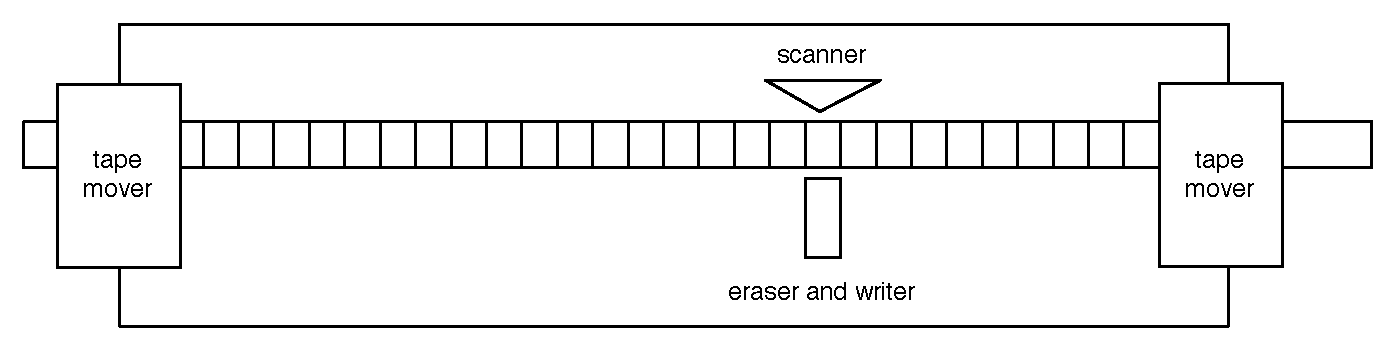
\includegraphics[width=0.9\textwidth]{turingmachine}
\caption{A Turing machine.}
\label{fig:machine}
\end{figure}


\begin{figure}
\centering
\subbottom[Turing Machine 1\label{fig:tm:tm1}]{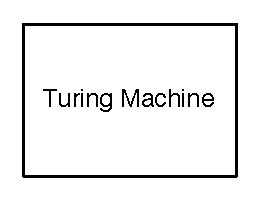
\includegraphics[width=0.2\textwidth]{block}}
\subbottom[Turing Machine 2\label{fig:tm:tm2}]{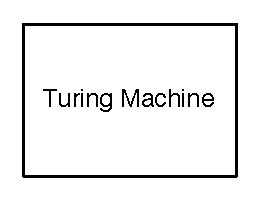
\includegraphics[width=0.2\textwidth]{block}}
\subbottom[Turing Machine 3\label{fig:tm:tm3}]{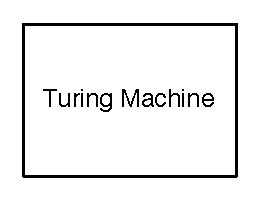
\includegraphics[width=0.2\textwidth]{block}}
\subbottom[Turing Machine 4\label{fig:tm:tm4}]{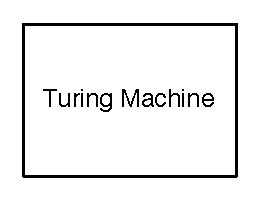
\includegraphics[width=0.2\textwidth]{block}}
\caption{Plots of four Turing machines}
\label{fig:tm}
\end{figure}




\section{Packages}
These packages might be helpful for writing your thesis:

\begin{description}
	\item[\texttt{caption}] to adjust the look of your captions
	\item[\texttt{glossaries}] for creating glossaries (also list of symbols)
	\item[\texttt{makeidx}] for indexes and the back of your document
	\item[\texttt{algorithm, algorithmicx, algpseudocode}] for adding algorithms to your document
\end{description}
\fi